\subsection{Discussion}
This section discusses the detected and manually-measured
solidification velocity results for each
of the two type of experiments outlined in the previous section.

% -------------------------------------------------------------------------
\subsubsection{AM Simulator}
% -------------------------------------------------------------------------
Rather than relying on the mean and median velocities to
assess the AM simulator detection procedure, the deviations from the mean
manual velocity were analyzed for each individual manual measurement
and for the detected velocities. This was repeated for each of the three
experiments to quantify the variance of the velocity as a way to
quantitatively compare the automated procedure to the manual measurements.
% 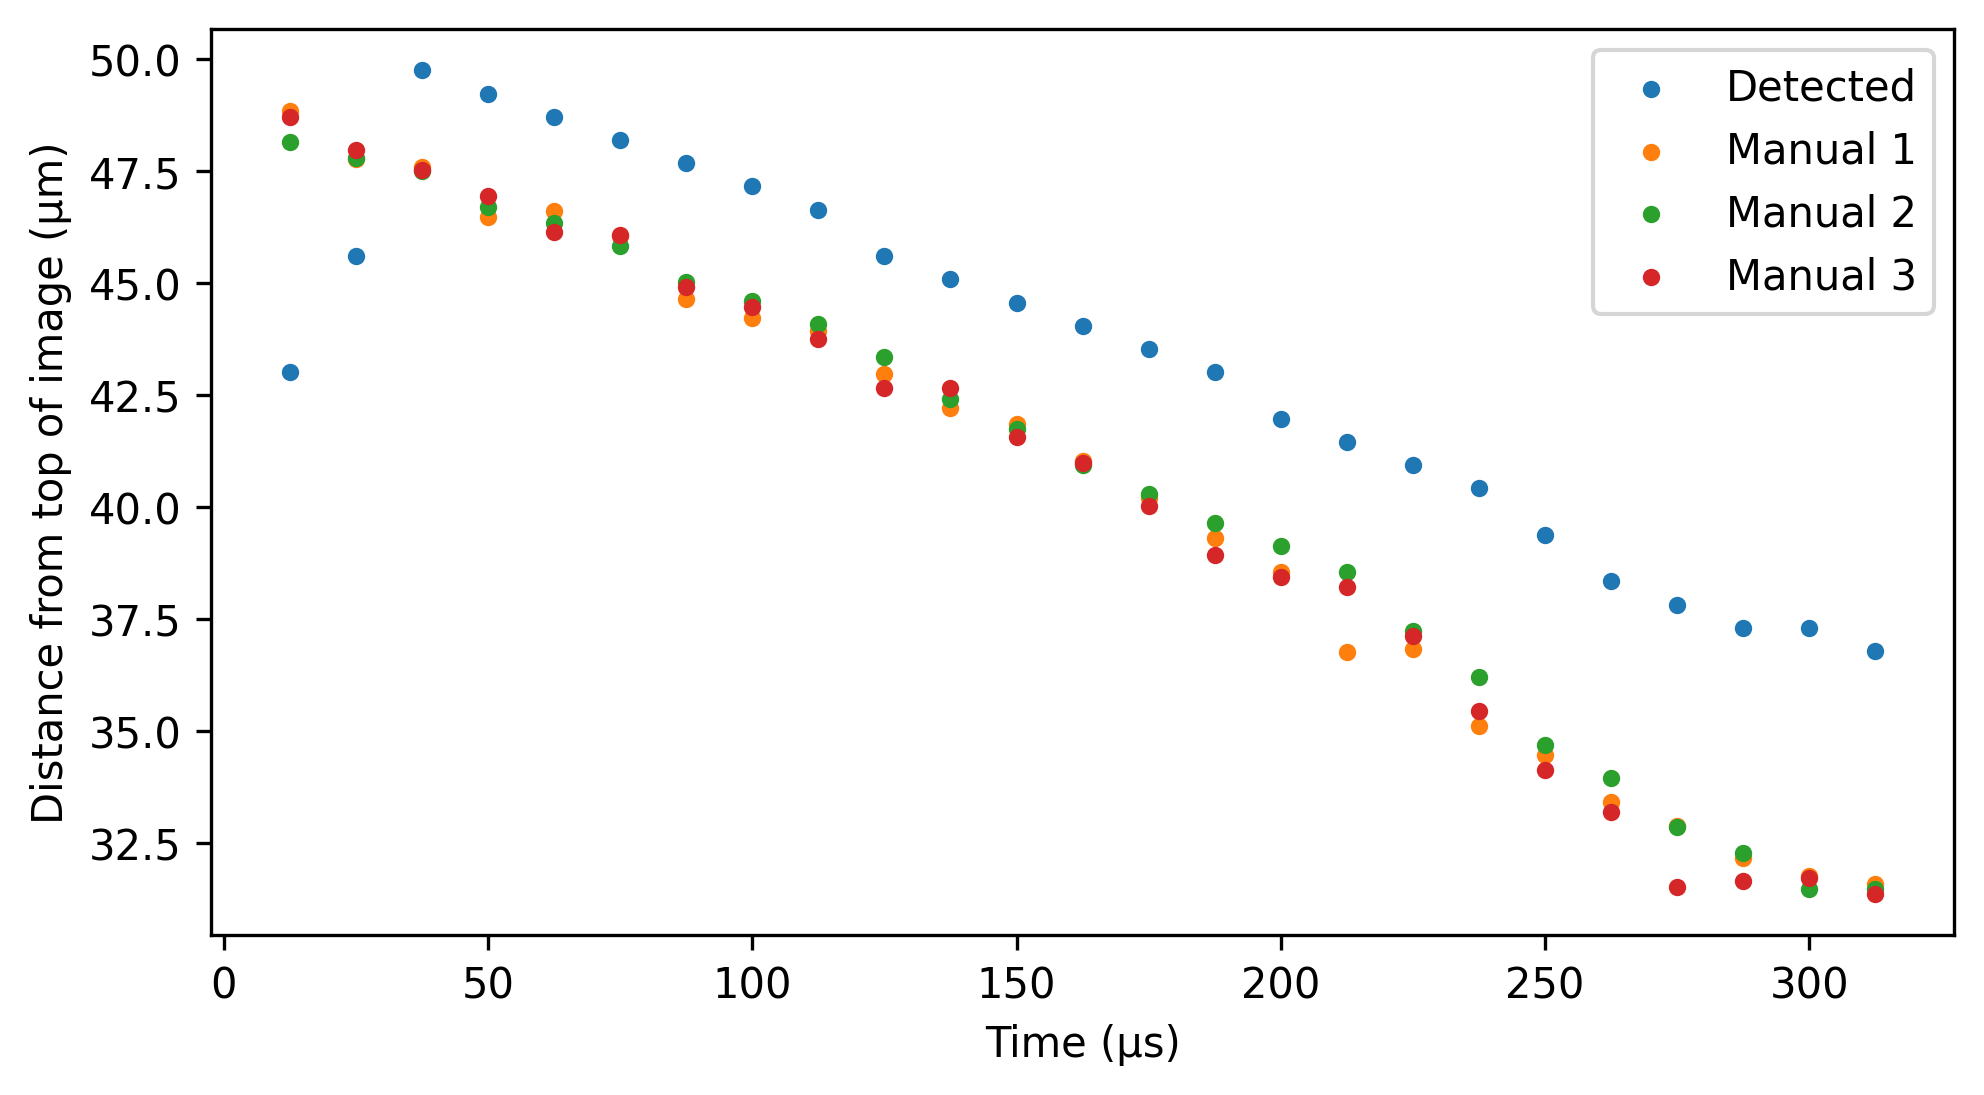
\includegraphics{figures/04/12-detected-vs-manual-1-10_shot05.png}
In the 104 W experiment, the mean velocities differ
drastically (0.021 m s\textsuperscript{-1} detected,
0.057 m s\textsuperscript{-1} manual), but less so
across the median values (0.041 m s\textsuperscript{-1} detected,
0.043 m s\textsuperscript{-1} manual),
suggesting there are outliers in the detected data that are skewing
the mean. This is further supported by the analyzing the average
deviations from the manual mean velocity (in terms of percent of the
manual mean: 78.800\% detected, 48.492\% manual). The average
deviations differ much like the mean velocities, however when considering
the spread of these deviations throughout the experiment, 58.333\% of
the manually measured velocities have a deviation lower than the average
manual deviation, whereas 87.5\% of the detected deviations are lower
than the same value. This indicates that the detected outliers are farther
from the manual mean than any of the individual manual measurements,
which is exemplified in \ref{fig/detected-aps-1} by the large
change in position (corresponding to a high velocity) across the first
three frames, compared to the more gradual change throughout the rest of the
experiment. This is especially interesting because the overall detected
interface position seems to be consistently about 2.5 µm higher than the
manually measured position. Since the interface still appears to be moving
at a rate similar to the manual measurements, this position discrepancy
could be the caused by the detection procedure capturing an optical artifact
slightly above the interface that nonetheless moved at the same rate.

% 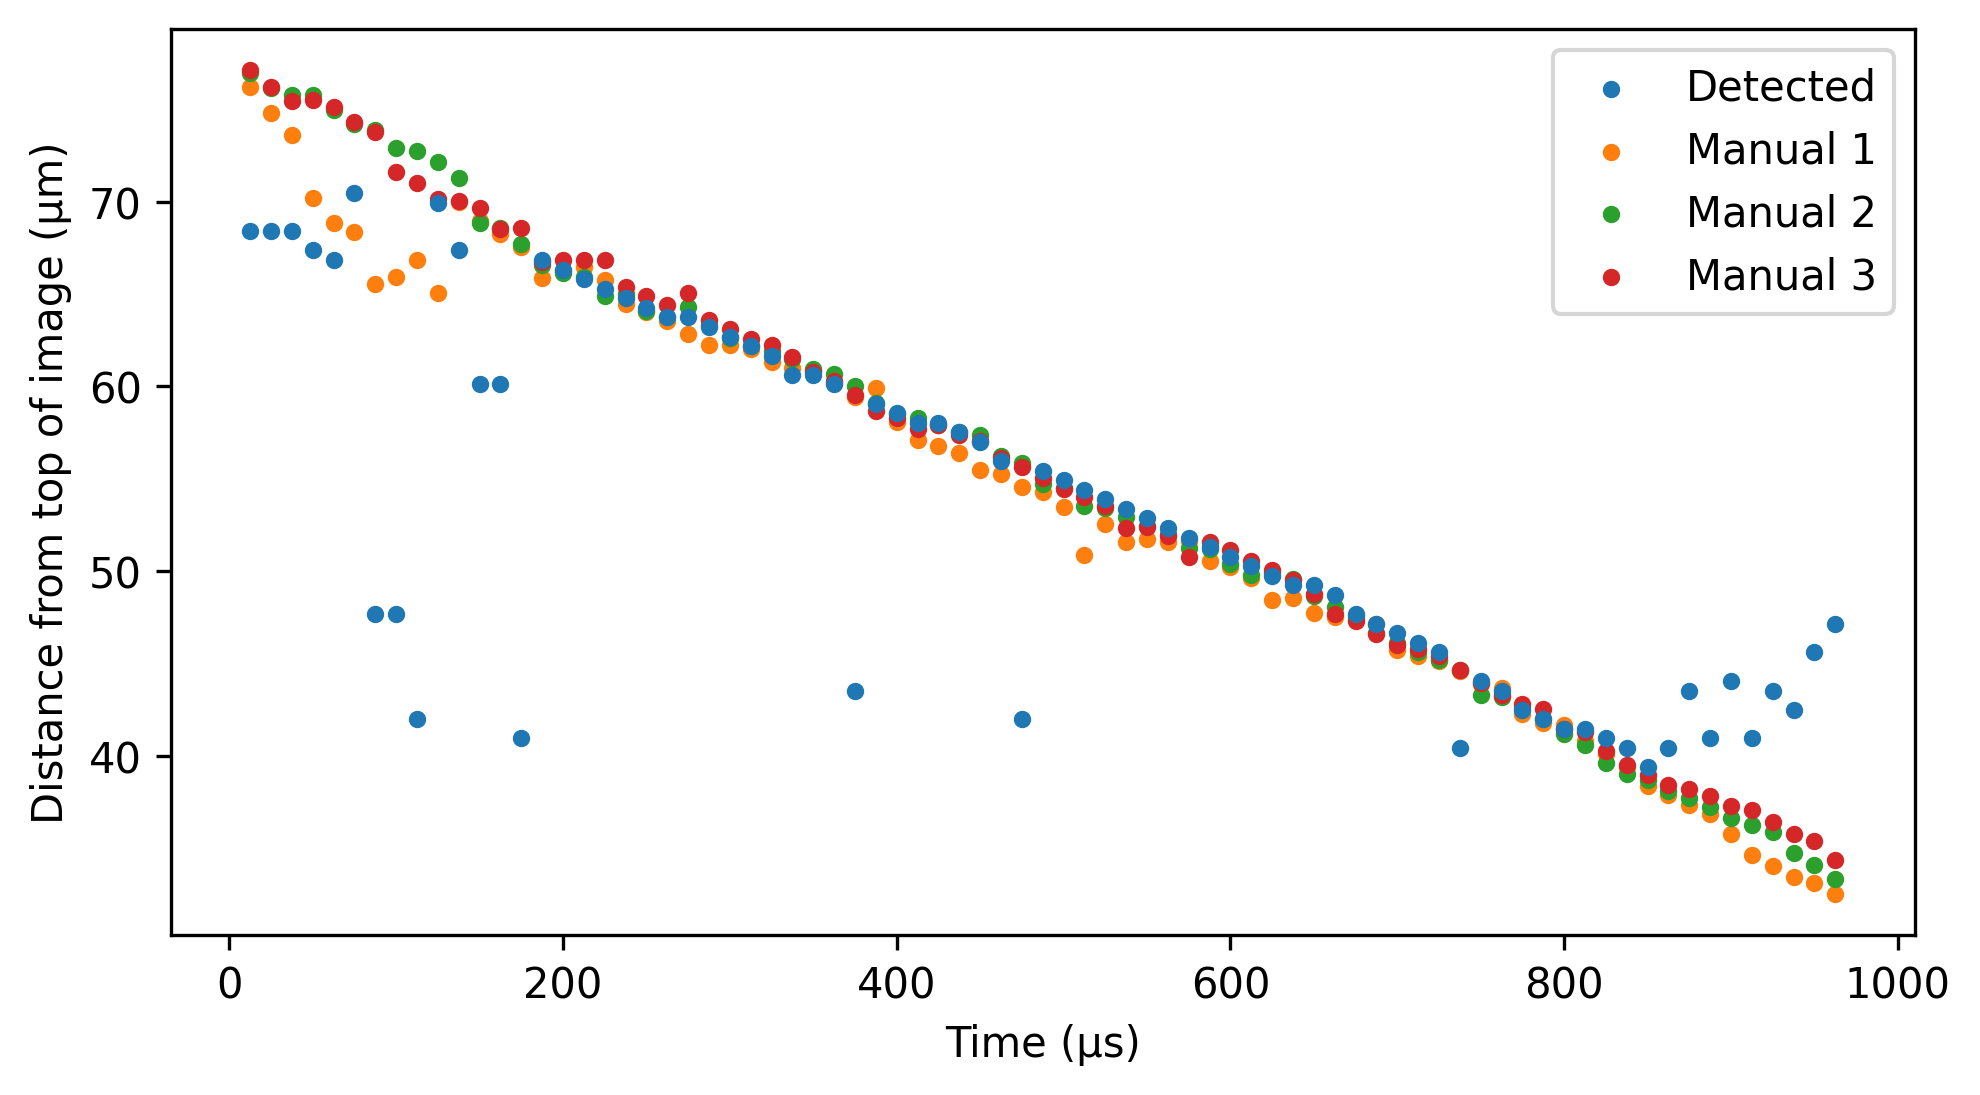
\includegraphics{figures/04/13-detected-vs-manual-2-06_shot01.png}
In the 156 W experiment, the average velocities differ
drastically (0.022 m s\textsuperscript{-1} detected,
0.046 m s\textsuperscript{-1} manual) but similar to
experiment 104 W less so across the median values
(0.041 m s\textsuperscript{-1} detected,
0.043 m s\textsuperscript{-1} manual).
The detected deviation from the manual mean
velocity is once again much larger than the manual deviation (in terms
of percent of the manual mean: 496.037\% detected, 69.798\% manual).
Considering the spread of these deviations yields slightly different
results in that 65.789\% of the manually measured velocities have a
deviation lower than the average manual deviation compared to the only
50.0\% of detected deviations. However, these 50.0\% of detected
deviations are also lower than half of the average manual deviation.
The outliers of the detected velocity may be further from the manual mean
than the manual measurements, but the fraction of the data that are
within the average manual deviation are much closer to the average than any
of the individual manual measurements. This can be seen in
\ref{fig/detected-aps-2} by the outliers of the detected positions
located farther away from the cluster of other data while the detected
positions closer to the rest of the data vary less across the frames than
the manual measurements. It is also worth noting that both the detected and
manual interface positions appear to be the most uncertain at the beginning
and end of the experiment, suggesting that the interface was harder to make
out than in the 104 W experiment, also supported by the fact that the
average manual deviation was higher for this experiment.

% 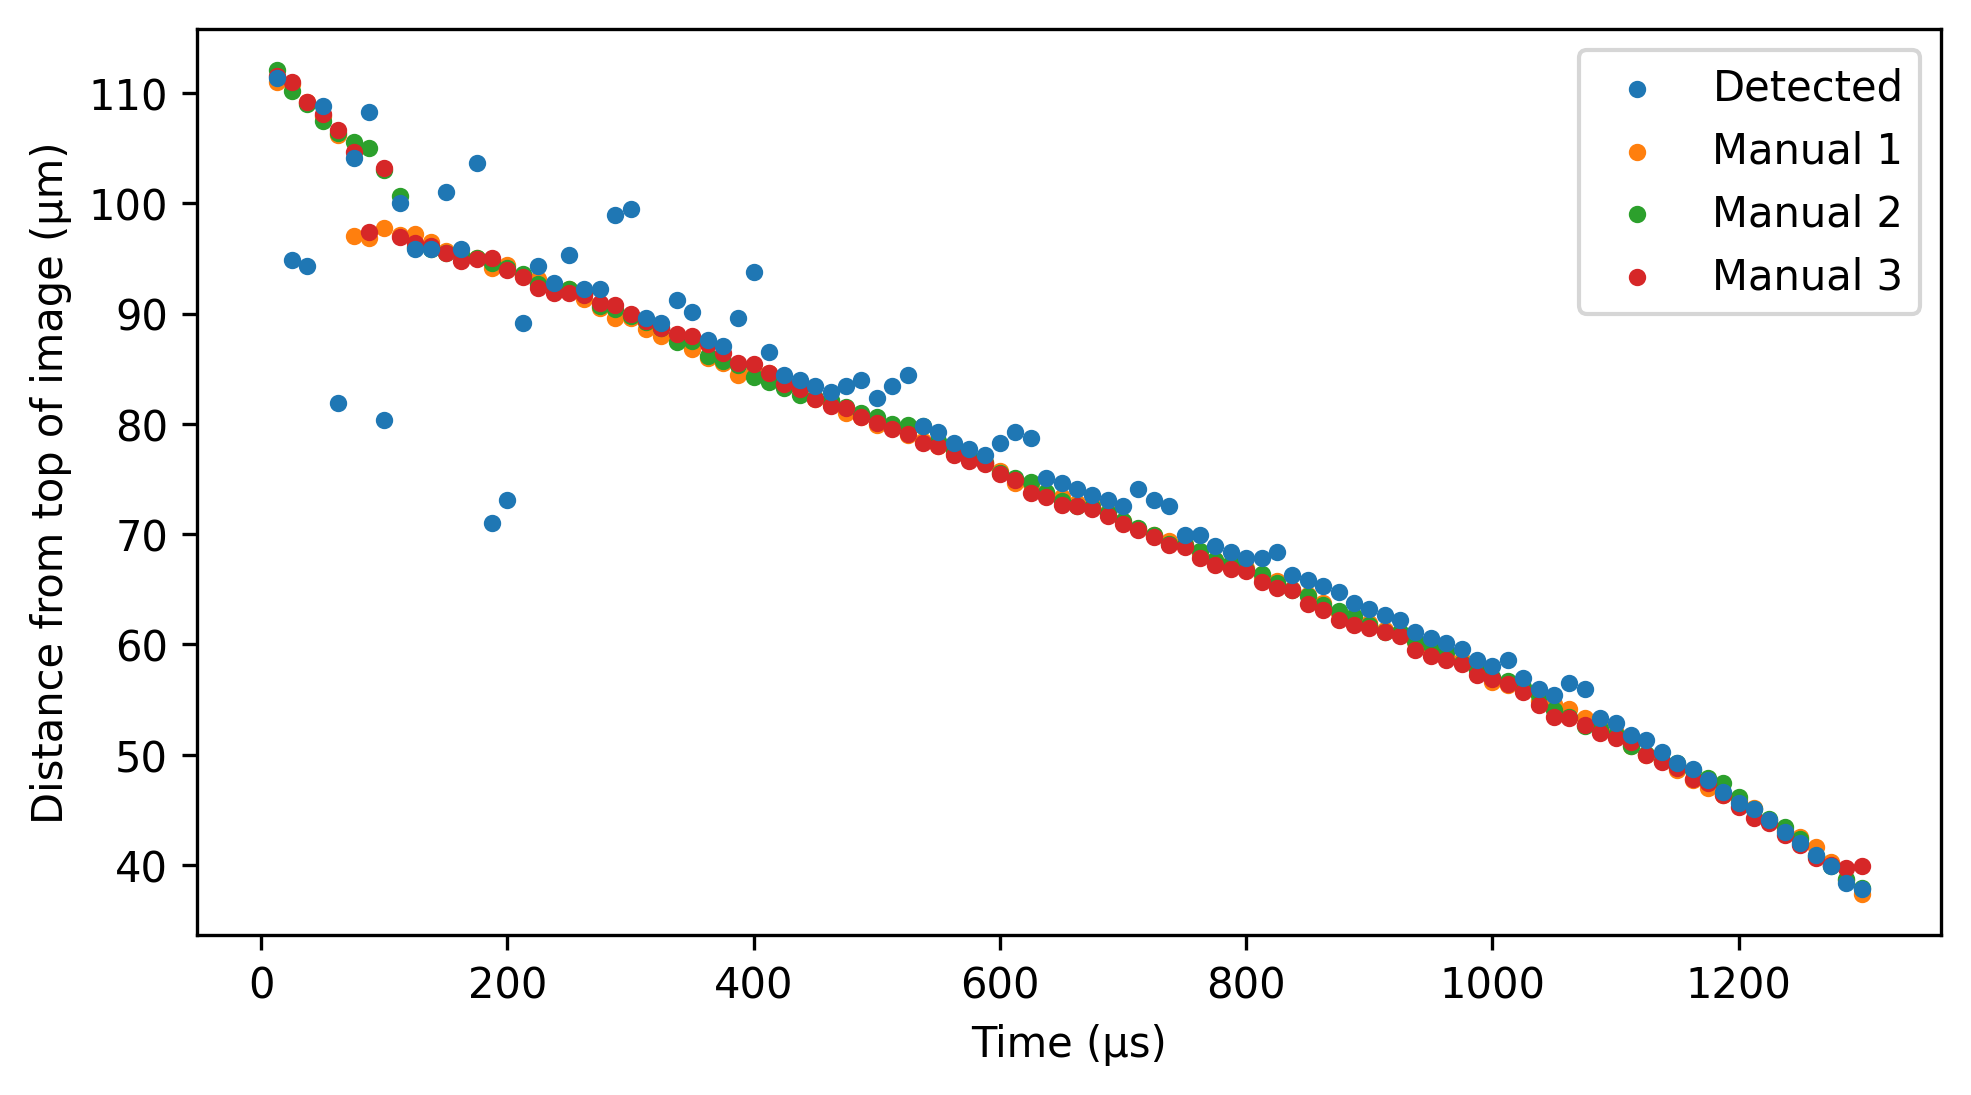
\includegraphics{figures/04/14-detected-vs-manual-3-12_shot01.png}
In the 208 W experiment, the mean velocities are
the same (0.057 m s\textsuperscript{-1} detected,
0.057 m s\textsuperscript{-1} manual). However, the median
values still differed (0.041 m s\textsuperscript{-1} detected,
0.052 m s\textsuperscript{-1} manual),
so the matching means is most likely an effect of the deviations
balanced on either side of the mean. Similar to the 156 W
experiment, the detected deviations from the manual mean velocity are much
higher than the manual measurements (in terms of percent of the
manual mean: 415.305\% detected, 56.777\% manual).
Much like the previous experiments, the outliers of the detected velocities
are much farther out from the rest of the data than the manually measured
velocities the experiment. 52.427\% of detected data has a deviation less
than the average manual deviation which is less than the 77.670\% of
the manually measured velocities, but still comparable. Comparing the data
that deviates within half the average manual deviation is even more similar
at 33.981\% of the detected velocities and 28.155\% of the manually
measured velocities. \ref{fig/detected-aps-3} shows the higher
deviation of the detected data far out from the mean like the previous
experiments, but a notable difference is that there appears to be a cusp in
the manually measured interface positions around 100 µs. This could be due
to a change in velocity of the S-L interface, but was more likely
due to a secondary interface that can appear in these experiments when a
melt pool becomes large enough to breach the edge of the sample. If the
sample breach happens at a different height than the minima of the melt pool,
the breach can appear to be a secondary interface. In this case, the breach
may have been more visible than the minima of the interface at the beginning
of the experiment. The first 100 - 200 µs of the experiment is also where
the detected position deviates from the mean the most.
As a side note, it is not entirely a coincidence that the median
velocity was the same for all
three experiments, as that value (0.041 m s\textsuperscript{-1})
corresponds to the 1 pixel/frame after converting pixels to µm with the
spatial resolution and frame number to µs with the experiment framerate.

% -------------------------------------------------------------------------
\subsubsection{Rapid Solidification}
% -------------------------------------------------------------------------
To assess the performance of the rapid solidification detection procedure,
the deviations from the mean manual
velocity were analyzed for the major and minor axes of the melt pools as
determined from each individual manual measurement
and for the detected procedure. This analysis was repeated for each of the
three DTEM experiments to characterize the performance of the procedure
compared to manual measurement.
% 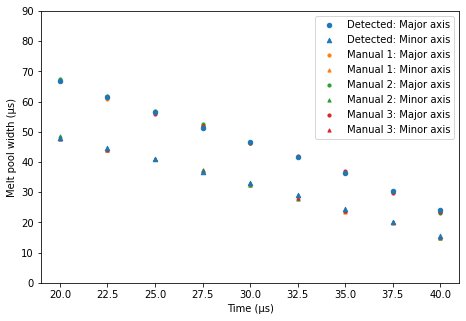
\includegraphics{figures/04/15-detected-vs-manual-03.png}
In the first experiment, the mean major / minor axis velocities
are similar (2.124 m s\textsuperscript{-1} / 1.619 m s\textsuperscript{-1}
detected, 2.183 m s\textsuperscript{-1} / 1.655 m s\textsuperscript{-1} manual),
and so are the median velocities
(2.167 m s\textsuperscript{-1} / 1.580 m s\textsuperscript{-1} detected,
2.101 m s\textsuperscript{-1} / 1.679 m s\textsuperscript{-1} manual).
The proximity of the mean to the medians for both the detected and manually
measured velocities suggests a small spread of the data, which is supported
by a lower deviation from the manual mean velocity (in terms of percent of the
manual mean for the major / minor axes: 7.9\% / 9.476\% detected,
13.543\% / 14.876\% manual). The data is distributed closely enough that it is
difficult to make out differences between the detected and manual data in
the plotted positions (\ref{fig/detected-dtem-1}).

% 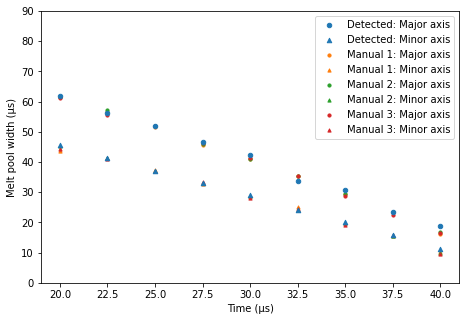
\includegraphics{figures/04/16-detected-vs-manual-04.png}
In the second rapid solidification experiment, the mean major / minor axis
velocities are also similar
(2.148 m s\textsuperscript{-1} / 1.719 m s\textsuperscript{-1} detected,
2.249 m s\textsuperscript{-1} / 1.725 m s\textsuperscript{-1} manual),
as are the median velocities
(2.028 m s\textsuperscript{-1} / 1.730 m s\textsuperscript{-1} detected,
2.318 m s\textsuperscript{-1} / 1.688 m s\textsuperscript{-1} manual).
The deviation from the manual mean velocity is also low (in terms of percent
of the manual mean for the major / minor axes:
24.001\% / 6.248\% detected, 10.331\% / 15.954\% manual),
however the deviation of the manual measurements is slightly larger,
as can be seen by some outliers in the the position data
(\ref{fig/detected-dtem-2}).

% 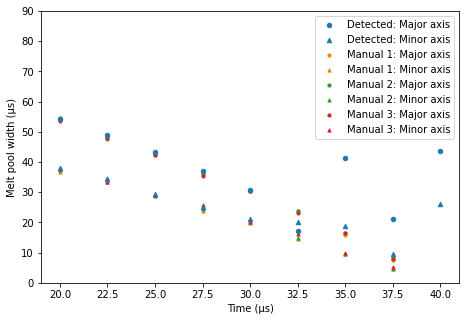
\includegraphics{figures/04/17-detected-vs-manual-09.png}
In the third rapid solidification experiment, the mean major / minor axis
velocities are (1.893 m s\textsuperscript{-1} / 1.628 m s\textsuperscript{-1}
detected, 2.640 m s\textsuperscript{-1} / 1.853 m s\textsuperscript{-1} manual),
and the median velocities
(2.494 m s\textsuperscript{-1} / 1.683 m s\textsuperscript{-1} detected,
2.561 m s\textsuperscript{-1} / 1.856 m s\textsuperscript{-1} manual).
The detected procedure had a larger deviation from the manual measurements
than in either of the two previous experiments. The deviations from the
manual mean velocity are much higher (in terms of percent of the manual
mean for the major / minor axes:
119.014\% / 42.621\% detected, 13.365\% / 14.290\% manual).
It is worth noting that in this experiment,
the manual measurements only recorded eight frames
in which the elliptical melt pool was manually measured because the sample
completely solidified before the last frame. As can be seen in the position
data, the detected melt pool size deviates more from the manual measurements
at the end of the experiment (\ref{fig/detected-dtem-3}).
This suggests the detection procedure is less effective when the melt pool is
near closing, most likely because the shape of the melt pool is lost within
the noise of the image.

